\chapter{Delay Differential Equations}

special case of more general functional differential equations (FDEs)

They often arise in automatic control %\cite
, where a controller montitors the state of a system in order to make control decisions to adjust this state.
If there is a delay between the observation and the control action, the differential equation describing the system not only depends on its current state, but also on its past.

need to specify in initial condition
at least for the time of longest delay

Even small delays can have a strong effect on the system's behaviour.
be both stabilizing and destabilizing
Stability is an important property for many applications.

Examples of ... which have been modeled using delay differential equations include epidemics, traffic flow and vibrations/chattering. See \cite{Falbo06FDEs} and there references therein.

Some methods to solve basic DDEs analytically are presented in \cite{Falbo06FDEs}.
numerical methods are not as 
see \cite{Bellen13NumericalDDEs}

\section{Piecewise Continuous Functions}
    \label{sec:piecewise-continuous-functions}
    
    The following definition is motivated by capturing the character evolution arising from hybrid systems. We will see that we can consider such to be piecewise continuous.
    function space of operation

    % \begin{definition}[Piecewise Continuous]\label{def:piecewise-continuous}
    %     Let $D=[a,b]\subseteq\R$ be a closed interval (this includes the cases when $a=-\infty$ or $b=\infty$, or both). The mapping $x:D\rightarrow\R^n$ is called \emph{piecewise continuous} if and only if there is a finite partition $\{t_i:i=\range{0}{m}\}$ of $D$ (i.e.\ $a=t_0<t_1<\ldots<t_m=b$) such that $x$ is continuous on each interval piece $[t_i,t_{i+1})$ for all $i=\range{0}{m-1}$ and the left sided limits
    %     \begin{equation}
    %         \lim_{\substack{t\upto t_{i+1}\\ t\in[t_i,t_{i+1})}} x(t)
    %     \end{equation}
    %     exist. Hence $x(b)$ can be an isolated point and this right interval limit $b$ is the only spot where such is allowed.

    %     We denote by $\Cnpw[0]{D}{\R^n}$ the set of \emph{piecewise continuous functions} on the compact interval $D$ (this excludes the cases with $\pm\infty$), mapping to $\R^n$.
    % \end{definition}

    \begin{definition}[Piecewise Continuously Differentiable]\label{def:pw-cont-diff}
        Let $D=\compactum{a}{b}\subseteq\R$ be a closed interval(this includes the cases when $a=-\infty$ or $b=\infty$, or both). The mapping $x\from D\to\R^n$ is called $n$-times \emph{piecewise continuously differentiable} if and only if there is a finite partition (ordered set) $\{t_i:i=\range{0}{m}\}$ of $D$ (i.e.\ $a=t_0<t_1<\ldots<t_m=b$) such that $x$ is $n$-times continuously differentiable on each interval $(t_i,t_{i+1})$ with \foreignlanguage{frenchb}{\emph{càdlàg} (\og continue à droite, limite à gauche\fg{})} derivative.

        This means that everywhere on $D$ the function and each of its derivatives are right continuous and have left limits.

        More precisely, for all $i=\range{0}{m-1}$ and for all $k=\range{0}{n}$ exist the left limits
        \begin{equation}
            \lim_{\substack{t\upto t_{i+1}\\ t\in(t_i,t_{i+1})}} \D[k]{x}(t)
        \end{equation}
        as well as the right limits
        \begin{equation}
            \lim_{\substack{t\downto t_{i}\\ t\in(t_i,t_{i+1})}} \D[k]{x}(t) = \D[k]{x}(t_i)
        \end{equation}
        which additionally coincide with the value of $\D[k]{x}$ at this knot $t_i$.

        Hence only $x(b)$ can be an isolated point and this right interval limit $b$ is the only spot where such is allowed.
        In the case $n=0$, we say $x$ is \emph{piecewise continuous}.

        For a compact interval $D\subset\R$ (this excludes the cases with $\pm\infty$), we denote by $\Cnpw[n]{D}{\R^n}$ the set of \emph{$n$-times piecewise continuously differentiable functions} on $D$ mapping to $\R^n$, and respectively, by $\Cnpw[0]{D}{\R^n}$ the set of\emph{piecewise continuous functions} on $D$.

        The supremum norm $\supnorm{\cdot}$ of the Banach space of continuous functions on the compactum $D$ can be extended to $\Cnpw[n]{D}{\R^n}$, since each element consists of a finite number of continuous parts.
    \end{definition}

    % FIXME: pw means as in def
    In the following
    in the sense of Definition~\ref{def:pw-cont-diff}.

    \begin{lemma}
        The composition of a continuous (outer) and a piecewise-continuous function (inner) is again piecewise-continuous with the same partition.
    \end{lemma}
    \begin{proof}
        The limits exist, because they commute with the continuous function and exist for the piecewise-continuous function.
    \end{proof}

    \begin{lemma}\label{lm:pc-integrable}
        A piecewise continuous function is (Riemann) integrable.
    \end{lemma}
    \begin{proof}
        This proof is usually given in every standard analysis book, see for example Theorem~6.10 in~\cite{Rudin76PrinciplesAnalysis} or Example~11.16b in~\cite{Gathmann12GDM}.
    \end{proof}

    The following lemma generalizes the fundamental theorem of calculus to piecewise continuous derivatives.

    \begin{lemma}\label{lm:pc-hauptsatz}
        Let $F\in\Cn[0]{\compactum{a}{b}}{} \cap \Cnpw[1]{\compactum{a}{b}}{}$
        % with the partition $\partition{a=t_0}{t_m=b}$
        with piecewise derivative $f$. Then
        \begin{equation*}
            F(t)-F(a) = \integral{a}{t} f(s)\dx[s]
            %\sum_{i=0}^k\int\limits_{t_i}^{t_{i+1}}f(t)\dx[t] + \int\limits_{t_k}^s f(t)\dx[t]
        \end{equation*}
        for all $t\in\compactum{a}{b}$.
        %where $t_k\leq s < t_{k+1}$.
        % FIXME: what about a=-inf or b=inf?
    \end{lemma}
    \begin{proof}
        On each interval $\compactum{t_{i-1}}{t_i}$ of the partition, $f$ is piecewise continuous and hence integrable.

        For all $\zeta\in\open{t_{i-1}}{t_i}$ is $F$ differentiable on $\compactum{t_{i-1}}{\zeta}$ with $\D{F}=f$.
        By the fundamental theorem of calculus (cf.\ standard analysis literature, e.g.~\cite{Gathmann12GDM,Rudin76PrinciplesAnalysis}), it follows
        \begin{equation*}
            \denseintegral{t_{i-1}}{\zeta} f(s)\dx[s] = F(\zeta)-F(t_{i-1})
        \end{equation*}
        and by the continuity of $F$ that
        \begin{equation*}
            \denseintegral{t_{i-1}}{t_i} f(s)\dx[s]
            = \lim_{\zeta\to t_i}\denseintegral{t_{i-1}}{\zeta} f(s)\dx[s]
            = \lim_{\zeta\to t_i} F(\zeta)-F(t_{i-1})
            = F(t_i)-F(t_{i-1})
        \end{equation*}
        For any $t\in\compactum{a}{b}$, there is a $k\in\set{\range{1}{m}}$ such that $t\in\closedopen{t_{k-1}}{t_k}$ (in the case $t=b$, set $k=m$), summation over $i=\range{1}{k}$ yields the telescoping series
        \begin{equation*}
            F(t)-F(a) = \sum_{i=1}^{k} \denseintegral{t_{i-1}}{t_i} f(s)\dx[s] + \integral{t_j}{t} f(s)\dx[s]
        \end{equation*}
        which is by the additivity of the integral
        \begin{equation*}
            F(t)-F(a) = \integral{a}{t} f(s)\dx[s]
        \end{equation*}
    \end{proof}

    \begin{figure}[t]\centering
        \begin{subfigure}[t]{0.48\textwidth}
            \centering
            \begin{tikzpicture}[line width=0.5pt, scale=(\textwidth-20pt)/2cm, >=Latex]

	% grid
	\draw[help lines, step=0.25, color=gray!30, dashed] (0,-0.5) grid (2,1);
	
	% axis
	\draw[->, thick] (0,0) -- (2,0); % x
	\draw[->, thick] (0,-0.5) -- (0,1); % y

	% ticks
	\draw (0,0) node[below right] {$t_0$};
	\draw[thick] (1,-0.03) -- (1,0.03);
	\draw (1,0) node[below] {$t_1$};

	
	\draw[curve,cadlag] plot[samples=50, smooth, domain=0:1] (\x, {((\x-2)^2-5*\x^3)/8});
	
	\draw[curve,leftp] plot[samples=50, smooth, domain=1:2] (\x, {(5*(\x-2)^2+\x^3)/8});

	% \filldraw[leftpoint] (0,0.5) circle (0.025);
	% \filldraw[rightpoint] (1,-0.5) circle (0.025);
		
	% \filldraw[leftpoint] (1,0.75) circle (0.025);
	

\end{tikzpicture}

            %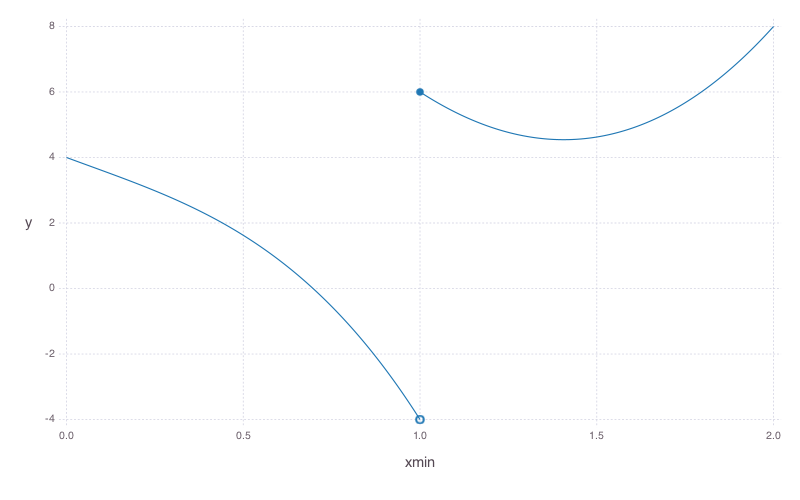
\includegraphics[width=\textwidth]{figures/allowed.png}
            \caption{Admissible piecewise continuous function.}
            \label{fig:allowed}
        \end{subfigure}
        \hfill
        \begin{subfigure}[t]{0.48\textwidth}
            \centering
            \begin{tikzpicture}[line width=0.5pt, scale=(\textwidth-20pt)/2cm, >=Latex]

	% grid
	\draw[help lines, step=0.25, color=gray!30, dashed] (0,-0.5) grid (2,1);
	
	% axis
	\draw[->, thick] (0,0) -- (2,0); % x
	\draw[->, thick] (0,-0.5) -- (0,1); % y

	% ticks
	\draw (0,0) node[below right] {$t_0$};
	\draw[thick] (1,-0.03) -- (1,0.03);
	\draw (1,0) node[below] {$t_1$};

	
	\draw[curve,cadlag] plot[samples=50, smooth, domain=0:1] (\x, {((\x-2)^2-5*\x^3)/8});
	
	\draw[curve,{Circle[width=4,length=4,fill=white]}-] plot[samples=50, smooth, domain=1:2] (\x, {(5*(\x-2)^2+\x^3)/8});

	% \filldraw[leftpoint] (0,0.5) circle (0.025);
	% \filldraw[rightpoint] (1,-0.5) circle (0.025);
	
	\filldraw[leftpoint] (1,0.4) circle (0.025);
	
	% \filldraw[rightpoint] (1,0.75) circle (0.025);
	

\end{tikzpicture}

            %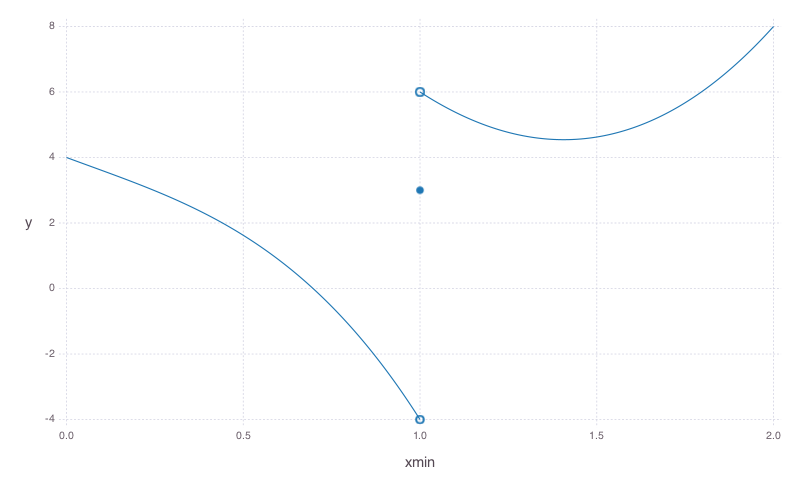
\includegraphics[width=\textwidth]{figures/not-allowed.png}
            \caption{Not allowed!}
            \label{fig:not-allowed}
        \end{subfigure}
        \caption{Examples to Definition~\ref{def:pw-cont-diff}.}
    \end{figure}


\section{Definition of DDEs}
    \label{sec:definition-dde}

    \cite{Roussel04DDEs}

    \begin{definition}[Delay Differential Equation]\label{def:dde}
        Given a function $f\from\deff\to\R^n$ and a set of time delays $0<\tau_1<\ldots<\tau_k$, a functional equation of the form
        \begin{equation}\label{eq:dde}
            \D{x}(t) = f(t,x(t),x(t-\tau_1),\ldots,x(t-\tau_k))
        \end{equation}
        is called (first order) \emph{delay differential equation} (DDE) with \emph{multiple constant, discrete delays} $\tau_j$.
        It is said to be \emph{autonomous} if its right hand side $f$ is time independent and \emph{pure}, if the right hand side only depends on $x(t-\tau_j)$ but not on $x(t)$.
        We define its \emph{maximal} and \emph{minimal delay} as $\taumax\defeq\tau_k$ and $\taumin\defeq\tau_1$, respectively.

        A DDE can be equipped with an \emph{initial condition} $x_{\tzero}$. It specifies the state, i.e.\ the values of $x$ on $[\tzero-\taumax, \tzero]$, on which the right hand side depends.
        Such a pair is called \emph{initial value problem} (IVP):
        \begin{equation}\label{eq:ivp}
            \begin{cases}
                \D{x}(t) = f(t,x(t),x(t-\tau_1),\ldots,x(t-\tau_k)) & \text{for } t\geq\tzero\\
                x(t) = x_{\tzero}(t) & \text{for } t\in\compactum{\tzero-\taumax}{\tzero}
            \end{cases}
        \end{equation}
    \end{definition}

    % TODO: autonomous DDEs is without loss of generality?
    In the following chapters, we will only consider autonomous DDEs, i.e.\ restrict to the case of initial time $\tzero=0$.

    % TODO: source for state-dependent and distributed delays
    The definition of a DDE can be extended to state-dependent or distributed delays (cf.~\cite{}). For simplicity, we restrict here to fixed delays, which already cover a wide range of applications.


%\section{Definition of Solution}
 %   \label{sec:definition-of-solution}

    \begin{definition}[Solution of DDE]\label{def:solution-dde}
    %there exists a $T>0$ such that
        A function $x\from\compactum{\tzero-\taumax}{\tzero+T}\to\R^n$ is called \emph{(local) solution} of the initial value problem~\eqref{eq:ivp}, if and only if
        $x$ obeys the initial condition
        \begin{equation*}
            x(t) = x_{\tzero}(t) \quad\text{for } t\in\compactum{\tzero-\taumax}{\tzero}
        \end{equation*}
        and $x$ is continuous and piecewise continuously differentiable on $\compactum{\tzero}{\tzero+T}$ fulfilling
        \begin{equation*}
            \D{x}(t) = f(t,x(t),x(t-\tau_1),\ldots,x(t-\tau_k))
        \end{equation*}
        on each (open) interval $(t_i,t_{i+1})$ of its partition $\Delta=\partition{\tzero=t_0}{t_m=\tzero+T}$ and
        \begin{equation*}
            \lim_{s\downto t_i}\D{x}(s) = f(t_i,x(t_i),x(t_i-\tau_1),\ldots,x(t_i-\tau_k))
        \end{equation*}
        in the knots $t_i$ for $i\in\set{\range{0}{m-1}}$.
        
        If the function $x$ is a solution for all $T>0$, it is called \emph{global}.   
    \end{definition}

    % FIXME: local solution is on a single subdiv int only -> cont diffable

    %TODO: Fortsetzbarkeit For example initial condition has jump, this point is limit for local solution.
    % FIXME: is this true? ref to source
    The left limit $\lim_{s\upto t_m}\D{x}(s)$ exists not necessarily in the last knot $t_m=\tzero+T$. If it does, the solution is continuable.

    % TODO: for the right-hand derivative?
    in knots: right sided derivative
    the right continuability of derivative is equivalent to right-hand derivative equals f


    \cite{Roussel04DDEs}
    If we limit $T$ by $\taumin$, we can see the solution of a delay differential equation as an operator mapping from functions on $\compactum{t-\taumax}{t}$ to functions on $\compactum{t}{t+\taumin}$.
    Then the solution of the initial value problem is the sequence of these functions.
    derivative not necessarily continuous at knots

% \begin{figure}[h]\centering
%     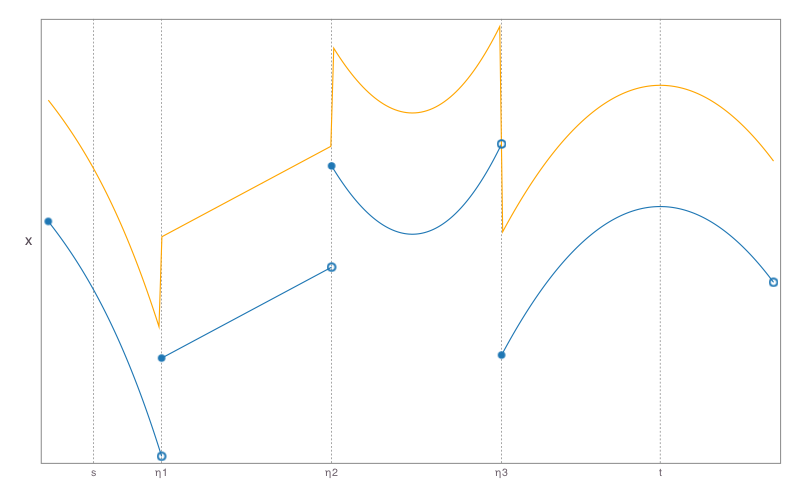
\includegraphics[width=\textwidth]{figures/multiple.png}
% 	\caption{Illustration of proof to Lemma \ref{lemma-continuity}}
% 	\label{fig:not-allowed}
% \end{figure}

% FIXME: This lemma is wrong. Show instead integrability of f(t,x_t)
%\begin{lemma}
%    \label{lemma-continuity}

    % Let $x:[\tzero-\tau,\tzero+T] \rightarrow \R^n$ be piecewise continuous (as in Definition \ref{definition-piecewise-continuous}) with the partition $\{t_0,\ldots,t_k\}$, i.e. there are $k$ subintervals.
    %
    % Then $t \mapsto x_t = x(t+\theta)$, where $\theta\in[-\tau,0]$, is a piecewise continuous mapping from $[\tzero,\tzero+T]$ into $\statespace[\tau]$.
%\end{lemma}

%\begin{proof}
    % $x$ is piecewise continuous and hence uniformly piecewise continuous on the compact interval $I=[\tzero-\tau,\tzero+T]$.
    % i.e. uniformely continuous on each subinterval with stetiger Fortsetzung in right side.
    % \begin{equation}
    %     \forall\epsilon >0 \exists\delta_i >0 \forall t,s\in I_i: \quad \abs{t-s}<\delta_i \Rightarrow \nnorm{x(t)-x(s)}<\epsilon
    % \end{equation}
    % Let $\epsilon > 0$. $x|_{[t_i,t_{i+1}]}$ (with stetiger fortsetzung in right interval limit) is uniformly continuous, i.e. there is a $\delta_i > 0$ (for the given $\epsilon$), such that $\forall\,t, s \in [t_i,t_{i+1}]$ holds
    % % TODO: can use \leq ?
    % \begin{equation}
    %     \abs{t-s} < \delta_i \Rightarrow \nnorm{x(t)-x(s)} < \epsilon
    % \end{equation}
    %
    % Among the given $\delta_i$, choose the smallest as $\delta = \min_i \delta_i$.
    %
    % For any $i$ and $s,t\in [t_i,t_{i+1})\subset [\tzero,\tzero+T]$ with $\abs{t-s}<\delta$, it holds
    % \begin{equation}
    %     \supnorm{x_t - x_s} = \sup_{\theta\in [-\tau,0]}\nnorm{x(t+\theta) - x(s+\theta)} < \epsilon
    % \end{equation}
    % since $t+\theta, s+\theta \in I$
    % Hence $t \mapsto x_t$ is uniformely continuous on $[t_i,t_{i+1})$.
%\end{proof}


\section{Method of Steps}
    \label{sec:method-of-steps}
    
    See \cite{Falbo06FDEs}
    by restricting the IVP onto an interval
    actually have an ODE IVP
    convert DDE into a ODE on a certain interval, by plugging the given initial condition into the delay differential equation, eliminating the explicit dependance on the past
    can be repeated on next interval by inserting the previously computed solution instead of the initial condition

    for $t\in [0,\tau]$, $x$ must satisfy the following ordinary initial value problem obtained by plugging the initial function into equation (??). For suitable $f$ and $x_0$, the existence (and uniqueness) of a solution on $[0,\tau]$ is guaranteed by ODE theory (\ldots{} or Picard-Lindelöf theorems).

    This procedure can then be applied repeatedly to extend the obtained solution by steps of length $\tau$.





\section{Existence and Uniqueness of Solutions}
    \label{solutions-existence-uniqueness}

    cannot have more than one solution
    under certain conditions, there is such 

    will consider rhs cont and lip
    $f$ Lipschitz with piecewise continuous initial function have existence and uniqueness ???? smoothing

    \begin{definition}[Lipschitz Continuity]\label{def:lipschitz}
        % similar to \cite{pruesswilke10GewDiffGl,Smith10IntroDDE}
        % FIXME: dont I need xtau in right side ??? 
        A function $f\from\deff\to\R^n$ is called \emph{(locally) Lipschitz continuous} (in its $i$-th argument) if and only if for all $a,b\in\R$ and $M>0$ there is a $L>0$ such that
        \begin{equation*}
            % TODO: is L(\nnorm*{x-x}+\nnorm*{y-y}) better? is equiv, with different L
            % FIXME: or just say Lipschitz continuous with respect to two other arguments, once for x once for y -> compare proof
            \nnorm*{f(t,x_1,\ldots,x_i,\ldots,x_k) - f(t,x_1,\ldots,y_i,\ldots,x_k)} \leq L\nnorm*{x_i - y_i}
        \end{equation*}
        for all $t\in [a,b]$ and $x_j,y_i\in\R^n$ with $\nnorm{x_j},\nnorm{y_i},\leq M$.
    \end{definition}

    \begin{lemma}\label{lm:bounded-lipschitz}
        Let $f\from\deff\to\R^n$ be continuous and Lipschitz continuous in all but its first argument.

        For any given compact interval $\compactum{a}{b}$ and $M>0$ there exists a bound $K>0$ such that
        \begin{equation}
            \nnorm{f(t,x_1,\ldots,x_k)}\leq K
        \end{equation}
        for all $t\in\compactum{a}{b}$ and $x_j\in\R^n$ with $\nnorm{x_j}\leq M$.
    \end{lemma}
    \begin{proof}
        Let $L_i$ be the Lipschitz constant for the $i$-th argument of $f$ on the given $\compactum{a}{b}$ and $M$. Set $L\eqdef\max_i\set{L_i}$. Then
        \begin{multline*}
            \nnorm{f(t,x_1,\ldots,x_k)} \leq \nnorm{f(t,x_1,\ldots,x_k) - f(t,0,\ldots,0)} + \nnorm{f(t,0,\ldots,0)}\\
            \leq L_i\nnorm{x_i-0} + \nnorm{f(t,0,\ldots,0)} \leq LM+P = K
        \end{multline*}
        for $t\in\compactum{a}{b}$ and $x_j\in\R^n$ with $\nnorm{x_j}\leq M$. We used the continuity of $f$ on the compact set $\compactum{a}{b}$ for the existence of
        \begin{equation*}
            P = \max_{s\in\compactum{a}{b}}\nnorm{f(s,0,\ldots,0)}
        \end{equation*}
    \end{proof}

    \begin{lemma}\label{lm:integral-equation}
        %TODO: compare with ODE lecture notes
        Finding a solution of the initial value problem~\eqref{eq:ivp} is equivalent to solving the integral equation
        \begin{equation*}\label{eq:integral-equation}
            \begin{cases}
                x(t) = x_{\tzero}(\tzero) + \integral{\tzero}{t} f(s,x(s),x(s-\tau_1),\ldots,x(s-\tau_k))\dx[s] & \text{for } t\geq\tzero\\
                x(t) = x_{\tzero}(t) & \text{for } t\in [\tzero-\taumax,\tzero]
            \end{cases}
        \end{equation*}
        where ... (same as for ivp)
        and is continuous in t.
        integral componentwise, f vector valued
    \end{lemma}
    \begin{proof}
        Let $x$ be a solution of the IVP. Thus $x$ is (by definition) piecewise continuous on $\compactum{\tzero-\taumax}{\tzero}$ andcontinuous and piecewise continuous differentiable on $\compactum{\tzero}{\tzero+T}$ with piecewise derivative $f(t,x(t),x(t-\tau_1),\ldots,x(t-\tau_k))$. This chain of a piecewise continuous and continuous function is piecewise continuous and hence by Lemma~\ref{lm:pc-integrable} integrable on $\compactum{\tzero}{\tzero+T}$.

        By Lemma~\ref{lm:pc-hauptsatz} it follows
        \begin{equation*}
            x(t) = x_{\tzero}(\tzero) + \integral{\tzero}{t} f(s,x(s),x(s-\tau_1),\ldots,x(s-\tau_k))\dx[s]
        \end{equation*}
        for $t\geq\tzero$.

        Conversely, let $x$ be a solution of the integral equation~\eqref{eq:integral-equation}.
        By the the fundamental theorem of calculus is $x$ continuous on $\compactum{\tzero}{\tzero+T}$ and differentiable in $t\in\compactum{\tzero}{\tzero+T}$ if $s\mapsto f(s,x(s),x(s-\tau_1),\ldots,x(s-\tau_k))$ is continuous in $s=t$.

         has the partition
        We define a partition of $\compactum{\tzero}{\tzero+T}$ by
        \begin{equation*}
            \mathcal{Z}\defeq\set{\tzero,\tzero+T}\cup\bigcup_{j=1}^{k}\bigcup_{\substack{i=1\\t_i\geq\tau_j}}^{m}\set{t_i-\tau_j}\defeq\partition{\hat{t}_0}{\hat{t}_p}
        \end{equation*}
        If $s\in\open{\hat{t}_{l-1}}{\hat{t}_l}$ then is $s-\tau_j\neq t_i$ for all $j$ and $i$. Hence the mapping $t\mapsto f(t,x(t),x(t-\tau_1),\ldots,x(t-\tau_k))$ is continuous in $t=s$, what implies that $x$ is differentiable in $s$ and that $\D{x}(s)=f(s)$.

        \begin{align*}
            \lim_{s\downto\hat{t}_l} \D{x}(s)
            &= \lim_{s\downto\hat{t}_l} f(s,x(s),x(s-\tau_1),\ldots,x(s-\tau_k))\\
            &= f(\hat{t}_l,x(\hat{t}_l),x(\hat{t}_l-\tau_1),\ldots,x(\hat{t}_l-\tau_k))
        \end{align*}
        by the continuity of $f$ and $\lim_{s\downto\hat{t}_l} x(s-\tau_j) = x(\hat{t}_l-\tau_j)$
        the limits exist
        \begin{equation*}
            \lim_{s\upto\hat{t}_l} \D{x}(s) = \lim_{s\upto\hat{t}_l} f(s,x(s),x(s-\tau_1),\ldots,x(s-\tau_k)) = 
        \end{equation*}
        Obviously, it obeys the initial condition, i.e. $x(t)=x_{\tzero}(t)$ for all $t\in\compactum{\tzero-\tau}{\tzero}$.
        % FIXME: f cont uberall in Voraussetzung?
    \end{proof}

    \begin{theorem}[Existence of unique solution]\label{thm:solution-existence}
        Consider the Delay Differential Equation
    %TODO: do we need global existence or just local?
        \begin{equation}
            \begin{cases}
                \D{x} = f(t,x(t),x(t-\tau)) & \text{for } t\geq\tzero\\
                x(t) = x_\tzero(t-\tzero)   & \text{for } t\in [\tzero-\tau,\tzero]
            \end{cases}
        \end{equation}
        with $f\from\deff\to\R^n$ continuous and satisfying the (local) Lipschitz condition in its second argument (Def.~\ref{def:lipschitz}).

        % where $\nnorm{\cdot}$ denotes the Euclidian norm on $\R^n$ and $\supnorm{\cdot}$ the supremum norm of the Banach space of continuous functions on $[-\tau,0]$.

        Then for each \emph{initial condition} $x_{\tzero}\in\statespace[\tau]$ and start time $\tzero$, there \textbf{exists} a \textbf{unique local solution} of the IVP on a time interval $[\tzero-\tau, \tzero+T]$. The duration $T>0$ depends on the sup-norm and discontinuity points of the initial condition. (?)
        This solution is continuous and piecewise differentiable on $\compactum{\tzero}{\tzero+T}$ with partition $t_i+\tau$.
    \end{theorem}

    The proof is smiliar to the proof of the existence theorem (Theorem 3.7) given in~\cite{Smith10IntroDDE}.
    \begin{proof}
        % FIXME: where sup-norm?
        As a piecewise continuous function, the initial condition can bounded by $M\geq \supnorm{x_\tzero}$ on $\delayinterval[-\tau]$.
        
        % FIXME: do I need t_0+tau or is just \tau okay? do I need x not to be pw, just cont in proof?
        If $\set{\range{-\tau=t_0}{t_k=0}}$ is the partition of $x_{\tzero}$, we choose $T=\min\set{t_0+\tau,\frac{M}{K}}$.
        
        % FIXME: M or 2M?
        Let $K>0$ be the upper bound for $f$ from Lemma~\ref{lm:bounded-lipschitz} on the set $S=[\tzero,\tzero+T] \times \{x\in R^n: \nnorm{x}\leq 2M\}\times \{y\in R^n: \nnorm{y}\leq 2M\}$ and $L>0$ the Lipschitz constant of $f$ for that set.

        % FIXME: why continuous? its pw cont? cont in tzero
        We construct a series $(x_{(m)})_{m\in\N_0}$ of piecewise continuous functions which approximates the solution of the initial value problem.
        Set
        \begin{equation}
            x_{(0)}(t)= \begin{cases}
                x_\tzero(0) & t\in [\tzero,\tzero+T]\\
                x_\tzero(t-\tzero) & t\in [\tzero-\tau,\tzero]
            \end{cases}
        \end{equation}
        For $m\in\N_{>0}$ define
        \begin{equation}
            x_{(m)}(t)= \begin{cases}
                x_\tzero(0) + \int_\tzero^t f(s,x_{(m-1)}(s),x_{(m-1)}(s-\tau))\dx[s] & t\in [\tzero,\tzero+T]\\
                x_\tzero(t-\tzero) & t\in [\tzero-\tau,\tzero]
            \end{cases}
        \end{equation}
        % FIXME: why exists integral? f cont, x in int even cont
        Integral exists
        It holds for all $m>0$ and $t\in \compactum{\tzero-\tau}{\tzero}$ by definition of the series
        \begin{equation}
            \nnorm*{x_{(m)}(t)-x_{(m-1)}(t)}=0
        \end{equation}
        We show by induction over $m$ that for all $t\in [\tzero,\tzero+T]$ it holds
        \begin{equation}
            \nnorm*{x_{(m)}(t)-x_{(m-1)}(t)} \leq \frac{K}{L}\frac{L^m (t-\tzero)^m}{m!}.
        \end{equation}
        Since obviously $\nnorm{x_{(0)}(t)}\leq M$, the statement for $m=0$ follows from the boundedness of $f$ on $S$ and the triangle inequality for integrals:
        \begin{equation}
            \nnorm{x_{(1)}(t)-x_{(0)}(t)} = \nnorm*{\int_\tzero^t f(s,x_{(0)}(s),x_{(0)}(s-\tau))\dx[s]} \leq K(t-\tzero)
        \end{equation}
        In the inductive step we can apply
        Since for any $m>0$, it holds by the triangle inequality and by the choice of $T$
        % FIXME: why x(m)(t) smaller than 2M, such that K holds?
        % TODO: why do integral and norm commute? once integral over vectors, once over scalars
        \begin{align}\label{eq:bounded-xm}
            \nnorm*{x_{(m)}} &\leq \nnorm*{x_\tzero(0)} + \int_\tzero^t \nnorm*{f(s,x_{(m-1)}(s),x_{(m-1)}(s-\tau))}\dx[s]\\
            &\leq M + K(t-\tzero) \leq M+KT\\
            &\leq 2M
        \end{align}
        if $\nnorm{x_{(m-1)}(t)}\leq 2M$.
        It follows by the Lipschitz property of $f$
        \begin{multline*}
            \nnorm*{x_{(m+1)}(t)-x_{(m)}(t)}=\\
            = \nnorm*{\int_\tzero^t f(s,x_{(m)}(s),x_{(m)}(s-\tau)) - f(s,x_{(m-1)}(s),x_{(m-1)}(s-\tau))\dx[s]}\\
            \leq L \int_\tzero^t \nnorm*{x_{(m)}(s) - x_{(m-1)}(s)}\dx[s]\\
            \leq \frac{L^m K}{m!} \int_\tzero^t (s-\tzero)^m\dx[s]
            = \frac{L^m K}{(m+1)!}(t-\tzero)^{m+1}
        \end{multline*}
        %We use this bound and the triangle inequality in
        The Cauchy criterion for convergent series (\cite{Gathmann12GDM} 6.13, \cite{Rudin76PrinciplesAnalysis} 3.22) applied to the exponential series states that
        \begin{equation*}
            % "\ " needed for space
            \mforall{\epsilon>0}\ \mexists{n_0\in\N_0}\ \mforall{m\geq k\geq n_0}\holds \sum_{i=k+1}^m \frac{(LT)^i}{i!} <\epsilon
        \end{equation*}
        So for any $\epsilon>0$ exist $k\in\N_0$ and $m\geq k$, such that
        \begin{align*}
            \nnorm*{x_{(m)}(t)-x_{(k)}(t)} \leq{} & \nnorm*{x_{(m)}(t)-x_{(m-1)}(t)} + \nnorm*{x_{(m-1)}(t)-x_{(m-2)}(t)} + {}\\
            & + \ldots + \nnorm*{x^{(k+1)}(t)-x^{(k)}(t)}\\
            \leq{} & \frac{K}{L}\frac{L^m (t-\tzero)^m}{m!} + \frac{K}{L}\frac{L^{m-1} (t-\tzero)^{m-1}}{(m-1)!} + {}\\
            & + \ldots +\frac{K}{L}\frac{L^{k+1} (t-\tzero)^{k+1}}{(k+1)!}\\
            \leq{} & \frac{K}{L}\sum_{i=k+1}^m \frac{(LT)^i}{i!} < \varepsilon
        \end{align*}
        for all $t\in [\tzero,\tzero+T]$, i.e. $x_{(m)}$ is a Cauchy sequence

    
        % FIXME: show that this a Cauchy series
        %This is the tail of the convergent exponential series and hence it converges to zero for $k\to\infty$ (boundedness and positivity of summands, monotonicity crit).

        % FIXME: why continuous? since integral exists
        Since $x_{(m)}$ is continuous on $[\tzero,\tzero+T]$, this Cauchy
        sequence admits a limit $x$ in the Banach space $\continuouss[0]{[\tzero,\tzero+T]}{\R^n}$ in terms of the supremum-norm.

        Again, we extend $x$ to $[\tzero-\tau,\tzero]$ with $x_\tzero$, such that $x\in\Cnpw[0]{[\tzero-\tau,\tzero]}{\R^n}$.


        

        Since by the continuity of the supremum norm it follows from~\eqref{eq:bounded-xm} that
        \begin{equation*}
            \supnorm*{x}=\lim_{m\to\infty}\supnorm*{x_m}\leq 2M
        \end{equation*}
        can apply Lipschitz property of $f$
        \begin{equation*}
            \sup_{t\in\compactum{\tzero}{\tzero+T}}\nnorm*{f(s,x_m(s),x_m(s-\tau))-f(s,x(s),x(s-\tau))} \leq \sup_{t\in\compactum{\tzero}{\tzero+T}}\nnorm*{x_m(t)-x(t)}
        \end{equation*}
        Due to the uniform convergence (conv in sup-norm) of $x_{(m)}\to x$, we get the uniform convergence
        \begin{equation*}
            f(s,x_m(s),x_m(s-\tau)) \xrightarrow{m\to\infty} f(s,x(s),x(s-\tau))
        \end{equation*}
        and hence the integral and the limit process swap and by
        \begin{align*}
            x(t) = \lim_{m\to\infty} x^{(m+1)} &= x_\tzero(0) + \lim_{m\to\infty}\int_\tzero^t f(s,x^{(m)}(s),x^{(m)}(s-\tau))\dx[s]\\
            &= x_\tzero(0) + \int_\tzero^t f(s,x(s),x(s-\tau))\dx[s]
        \end{align*}
        it follows that $x$ solves the integral equation and hence, by Lemma~\ref{lm:integral-equation},
        this proves the existence of a solution to the DDE.
        % TODO: continuous because limit in Banach space, diffable and subdiv see integral equiv lemma

        % TODO: can one solution be on [\tzero, T_2] with T_2<T ?
        It remains to show uniqueness.
        Let $x$ and $\bar{x}$ be two solutions of the DDE on $[\tzero,\tzero+T]$.
        By Lemma \ref{lm:integral-equation} they are equivalent to solutions of the integral equations
        \begin{equation}
            x(t) = x_\tzero(0) + \int_\tzero^t f(s,x(s),x(s-\tau))\dx[s]
        \end{equation}
        and
        \begin{equation}
            \bar{x}(t) = x_\tzero(0) + \int_\tzero^t f(s,\bar{x}(s),\bar{x}(s-\tau))\dx[s]
        \end{equation}
        For $t\in [\tzero,T]$, we set
        \begin{align*}
            \rho(t) &:= \nnorm*{x(t)-\bar{x}(t)} \leq \int_\tzero^t \nnorm*{f(s,x(s),x(s-\tau))-f(s,\bar{x}(s),\bar{x}(s-\tau))}\dx[s]\\
            & \leq L \int_\tzero^t \nnorm*{x(s)-\bar{x}(s)}\dx[s] = L \int_\tzero^t \rho(s)\dx(s)\\
            &= L \int_\tzero^t \e{-\alpha s}\rho(s)\e{\alpha s}\dx[s] \leq L \sup_{s\in [\tzero,\tzero+T]}\left(\e{-\alpha s}\rho(s)\right)\int_\tzero^t \e{\alpha s}\dx[s]\\
            & \leq\frac{L}{\alpha}\e{\alpha t} \sup_{s\in [\tzero,\tzero+T]}\left(\e{-\alpha s}\rho(s)\right)
        \end{align*}
        with $L$ the Lipschitz constant of $f$ on the set ...
        and $\rho$ is continuous, since $x$ continuous
        Choosing $\alpha=2L$ and multiplying with $\e{-\alpha t}>0$ leads to
        \begin{equation}
            \rho(t)\e{-2Lt} \leq \frac{1}{2}\sup_{s\in [\tzero,\tzero+T]}\left(\e{-2L s}\rho(s)\right)
        \end{equation}
        for all $t\in [\tzero,\tzero+T]$
        \begin{equation}
            0 \leq \sup_{t\in [\tzero,\tzero+T]}\left(\rho(t)\e{-2Lt}\right) \leq \frac{1}{2}\sup_{s\in [\tzero,\tzero+T]}\left(\e{-2L s}\rho(s)\right)
        \end{equation}
        That is only possible if $\rho(t)=0$ for all $t\in [\tzero,\tzero+T]$, which means $x(t)=\bar{x}(t)$.

        % TODO: still needed?
        just proof existence/uniqueness on each peace of continuity proof continuity at knots with Lemma of integral equ

    \end{proof}

% TODO: on [\tzero,t_1] DDE equiv to ODE/IntEq
% -> ex unique sol on [\tzero, t_1]
% -> ex unique sol on [\tzero,\tau] (glob Lip of f on [tzero,tau])
% -> ex unique sol on [\tzero,2\tau] (continuous?, diffable?)
% show continuity and pw diffable (nth to show)
    % \begin{lemma}[cont]\label{lm:c}
    %     $x_1$ loc sol on $\compactum{\tzero-\tau}{\tzero+t_1}$ for init cond $x_{\tzero}$
    %     $x_2$ and loc sol on $\compactum{\tzero+t_1-\tau}{\t_1+T}$ for init cond $x_1$
    %     then $x_1(\tzero+t_1)=x_2(\tzero+t_1)$
    %     follows from initial cond $x_1$
    % \end{lemma}
\begin{corollary}
    \label{cor:continuability-of-solution}

    % TODO: What is derivation in randpunkten of interval [] ?
    If in Theorem \ref{theorem-solution-existence} $T=t_1-\tau$, can reapplay theorem with starting point $\tzero=\tzero_{old}+t_1-\tau$. Get existence of unique solution on $[\tzero-\tau,\tzero+S]$ with $S>T$.
\end{corollary}

\begin{corollary}
    \label{corollary}
    If f is polynomial in $t$, $x(t)$ and $x(t-\tau)$ then theorem holds

    polynomial -> continuously differentiable -> locally Lipschitz
% IDEA: can show? init cond bounded by M, and loc sol bounded by M, get glob sol since f glob Lip on set of bounded inputs?


    %TODO: put after uniqueness theorem, need uniqueness and existence so that amap well-defined
    The notion of solution for an autonomous DDE as given above can be lifted to be a trajectory $\trajectory[x]$ in the statespace
    \begin{equation}
        \trajectory[x] \from [0,T] \to \statespace[\tau],\\
        t \mapsto \xbartaut{t}
    \end{equation}

    The \emph{state} at time $t$ is a function which provides a time limited history up to the current time. This is all information needed to determine (using the DDE) to determine the solution for time $\geq t$. It is defined as $\xbartaut{t}(s)\defeq x(t+s)$ for $s\in [-\tau,0]$. In the case of $t=0$, we simplify the notation to $\xbartau \defeq \xbartaut{0}$.
    This notion of solution is a \emph{dynamical systems} point of view which later turns out to be useful.

  Other results know from ordinary differential equations can be adapted to delay differential equations, such as continuous (or even differentiable) dependence of the solution on initial data and, see \cite{Dads06DDEs} % TODO: add other cites

%TODO: can write DDE (eq??) from definition as

\begin{equation}
    \begin{cases}
        \D{x}=f(\xbartaut{t})\defeq g(\xbartaut{t}(0),\xbartaut{t}(-\tau)) &\text{for } t\geq 0\\
        x(t)=x_0(t) & \text{for } t\in[-\tau,0]
    \end{cases}
\end{equation}
\end{corollary}

\begin{proof}

\end{proof}

% TODO: non-autonomous -> autonomous

\begin{example}
    Delay differential equations can often incorporate a much richer behaviour than ordinary differetial equations.
    The basic ODE IVP
    \begin{equation}
        \begin{cases}
            \D{x}(t) = -x(t)\\
            x(0) = x_0
        \end{cases}
    \end{equation}
    has the solution $x(t)=x_0 e^{-t}$. However the similiar DDE
    \begin{equation}
        \begin{cases}
            \D{x}(t) = -x(t-\tau) & t\geq 0\\
            x(t) = x_0(t) & -\tau\leq t\leq 0
        \end{cases}
    \end{equation}
    has a much richer dynamics, but solution (as series) for $x_0\equiv 1$, can compute first solutions by method of steps. \ldots{}    
\end{example}


\begin{figure}[h]\centering
    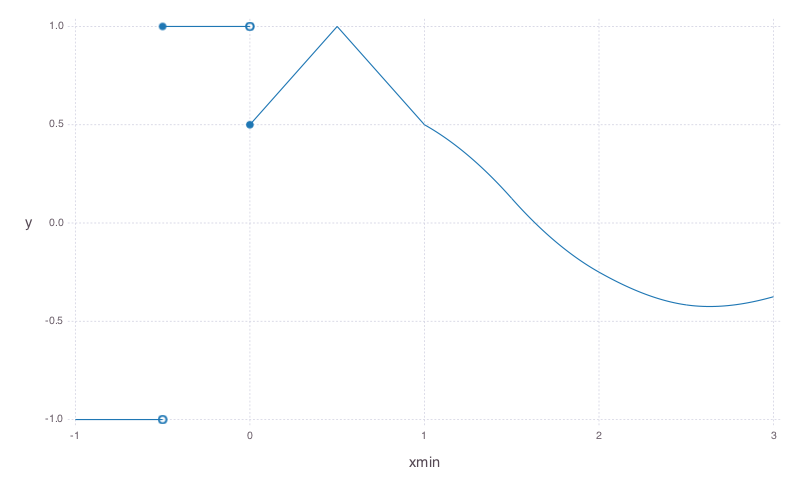
\includegraphics[width=\textwidth]{figures/piecewise-initial-function.png}
	%\caption{}
	\label{Piecewise continuous initial function.}
\end{figure}

